\section{Kuberenetes}

\begin{figure}
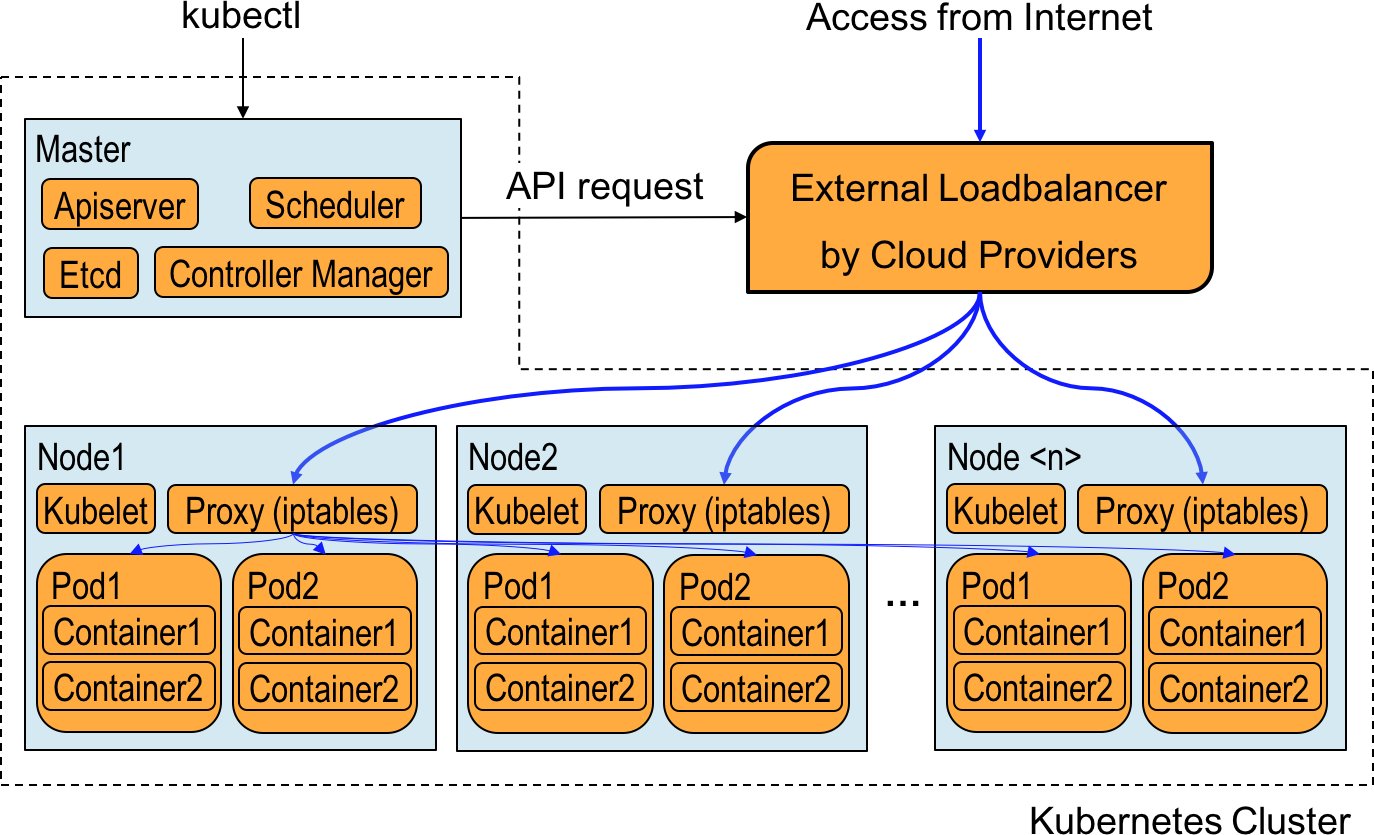
\includegraphics[width=\columnwidth]{Figs/K8sConventional}
\caption{Conventional architecture of a Kubernetes cluster.}
\label{fig:K8sConventional}
\end{figure}

Problems commonly occur when the Kubernetes container management system is used outside of recommended cloud providers(such as GCP or AWS).
Figure~\ref{fig:K8sConventional} shows an exemplified Kubernetes cluster.
A Kubernetes cluster typically consists of a master and nodes. They can be physical servers or VMs.
On the master, daemons that control the Kubernetes cluster are typically deployed. 
These daemons include, apiserver, scheduler, controller-manager and etcd. 
On the nodes, the kubelet daemon will run {\it pods}, depending the PodSpec information obtained from the apiserver on the master.
A {\em pod} is a group of containers that share same net name space and cgroups, 
and is the basic execution unit in a Kubernetes cluster.

When a service is created, the master will schedule where to run {\em pods} and kubelets on the nodes will launch them accordingly.
At the same time, the masters will send out requests to cloud provider API endpoints, asking them to set up external cloud load balancers.
The proxy daemon on the nodes will also setup iptables DNAT\cite{MartinA.Brown2017} rules. 
The Internet traffic will then be evenly distributed by the cloud load balancer to nodes, 
after which it will be distributed again by the DNAT rules on the nodes to the designated {\em pods}. 
The returning packets will follow the exact same route as the incoming ones.

This architecture has the followings problems: 
1) Having cloud load balancers whose APIs are supported by the Kubernetes daemons is a prerequisite.
There are numerous load balancers which is not supported by the Kubernetes.
These include the bare metal load balancers for on-premise data centers.  
In such cases, users are required to set up the routing manually depending on the infrastructure.
The traffic would be routed to a node then distributed by the DNAT rules on the node to the designated {\em pods}.
However, this approach significantly degrades the portability of container clusters.

2) Distributing the traffic twice, first on the external load balancers and second on each node, 
complicates the administration of packet routing. 
Imagine a situation in which the DNAT table on one of the nodes malfunctions.
In such a case, only occasional timeouts would be observed, which would make it very difficult to find out which node was malfunctioning.   

In short, 1) Kubernetes can be used only in limited environments where the external load balancers are supported, 
and 2) the routes incoming traffic follow are very complex.

In order to address these problems, we propose a containerized software load balancer 
that is deployable in any environment even if there are no external load balancers.

\section{Overlay Network}\label{sec:overlay_network}

In order to discuss load balancer redundancy, the knowledge of the overlay network is essential.
We briefly explain an abstract concept of overlay network that is common to existing overlay network including flannel\cite{coreos_2018} and calico\cite{project_calico}.

\begin{figure}[tb]
\begin{center}
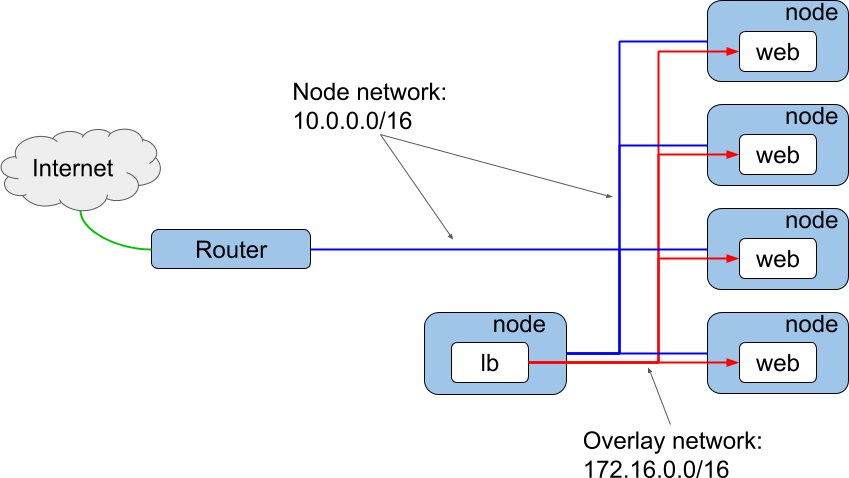
\includegraphics[width=\columnwidth]{Figs/overlay.png}
\end{center}
\caption{
  The network architecture of an exemplified container cluster system. %\\ %\par
  A load balancer(lb) pod(the white box with "lb") and web pods are running on nodes(the blue boxes).
  The traffic from the internet are forwarded to the lb pod by the upstream router using the node network,
  and the distributed to web pods using the overlay network.
}
\label{fig:overlay}
\end{figure}

Fig.~\ref{fig:overlay} shows schematic diagram of network architecture of a container cluster system. 
Suppose we have a physical network(node network) with IP address range of 10.0.0.0/16 and an overlay network with IP address range of 172.16.0.0/16.
The node network is the network for nodes to communicate with each other.
The overlay network is the network setups for containers to communicate with each other.
An overlay network typically consists of appropriate routing tables on nodes, and optionally of tunneling setup using ipip or vxlan.
The upstream router usually belongs to the node network.
When a container in the Fig.~\ref{fig:overlay} communicates with any of the nodes, it can use its IP address in 172.16.0.0/16 IP range as a source IP, since every node has proper routing table for the overlay network.
When a container communicates with the upstream router that does not have routing information regarding the overlay network, the source IP address must be translated by Source Network Address Translation(SNAT) rules on the node the container resides.

The SNAT caused a problem when we tried to co-host multiple load balancer containers for different services on a single node, and let them connect the upstream router directly.
This was due to the fact that the BGP agent used in our experiment only used the source IP address of the connection to distinguish the BGP peer.
The agent behaved as though different BGP connections from different containers belonged to a single BGP session because the source IP addresses were identical due to the SNAT.

\subsection{Flannel}
\paragraph{\bf host-gw}
\paragraph{\bf vxlan}
\paragraph{\bf udp}

\subsection{Calico}
\paragraph{\bf no-tunnel}
\paragraph{\bf ipip}

\section{Multicore Packet Proccessing}
\subsection{rss}
\subsection{rps}
\subsection{Others}
\paragraph{rfs}
\paragraph{xps}
\paragraph{xfs}

\section{Other parameters}
\subsection{tcp congestion mode}

\section{Cloud Load Balancers}
\subsection{Maglev}
\subsection{Ananta}
\subsection{GCP Load Balancer}
GCP experimental data.
